\documentclass[10pt]{article}

%packages

\usepackage{titlesec}
\usepackage{titling}
\usepackage[margin=0.5in] {geometry}
\usepackage{multicol}
\usepackage{hyperref}
\usepackage{graphicx}


%section

\titleformat{\section}
{\Large \bfseries \uppercase}
{\hspace{-.25in}\thesection}
{0em}
{. }[\titlerule]


%sub Section

\titleformat{\subsection}
{\bfseries\large}
{$\bullet$}
{0em}
{ }

%sub Sub Section

\titleformat{\subsubsection}[runin]
{\bfseries}
{}
{0em}
{-}  

\titlespacing{\subsubSection}
{0em}{0em}{0em}


%make titile

\renewcommand{\maketitle}{
\begin{center}
{\LARGE\bfseries
\theauthor}

\vspace{.25em}
\line(1,0){250}
\end{center}
\begin{multicols}{2}
\noindent
%address
Fl.No. 11/A,\\
Hariangan Society,\\
Near New Life Hospital,\\
Gurudwara Chowk,\\
Akurdi,Pune -411044\\

\columnbreak
\begin{flushright}
Contact: +91-7798497481\\
E-mail Id: aditya.bichave@gmail.com\\
Github: \url{https://github.com/Aditya-Bichave}
\end{flushright}
\noindent
\hspace{10em}
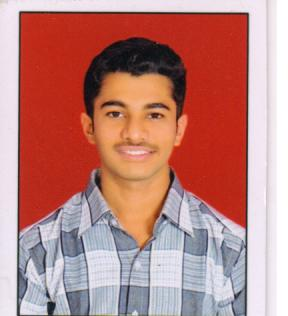
\includegraphics[width = 8em]{Aditya.jpg}

\end{multicols}



}





















\begin{document}

\title{Resume}
\author{Aditya Bichave}
\maketitle

\section{Objective}

To seek a challenging position as a Machine Learning Engineering with an organization of repute, where I can utilize my skills and knowledge of Computer Science concepts and advance technologies like Deep Learning, Image processing.

\section{Education}

\begin{tabular}[8pt]{| c | c | c | c | c |}
\hline
	Degree & College/School & University & passing year & Pass Percentage\\
\hline
	B.E Computer Engineering & Pimpri Chinchawad College of Engineering ,Pune & SPPU & 2021 & -- \\
\hline
	H.S.C & Ashoka Universal School and Jr.College,Nashik & ISC & 2017 & 83.60 \\
\hline
	S.S.C & Sacred Heart Convent High School, Nashik & S.S.C & 2015 & 91.00\\
\hline
\end{tabular} 

\section{Projects}
	


\section{Training \& Internship}

\section{Research publications}

\section{Technical Skills}
	\subsection{Languages:}
		\subsubsection{Programming Languages: }
			C, C++, Python, Java.
		\subsubsection{Markup Languages:}
			HTML,CSS,XML
		\subsubsection{Tools}
			PyTorch,Tensorflow,Keras, OpenCV,Android Studio,Atmel Studio,Arduino

\section{Soft Skills}
	\begin{multicols}{2}
	\begin{itemize}
	\item Confident \\
 	\item Problem Solving\\
	\item Motivated\\ 
	\item Curious\\
	\columnbreak
	\item Persistent \\
	\item Teamwork\\
	\item Self-managment\\
	\end{itemize}
	\end{multicols}


\section{Extra-curricular Activities}



\section{co-curricular activities}



\section{Personal Details} 
\begin{itemize}

\item{Father's Name: Anand Bichave}
\item{Mother's NAme: Rashmi Bichave}
\item{Sex: Male}
\item{Date Of Birth: 9th April, 1999}
\item{Nationality: Indian}
\item{Marital Status: Single}

\end{itemize}






\end{document} 